\documentclass[a4paper,onecolumn,final,10pt]{memoir}

% -------- %
% Preamble %
% -------- %

\usepackage[stretch=10]{microtype}
\usepackage[utf8]{inputenc}
\usepackage[british]{babel}
\usepackage{csquotes}
\usepackage[a4paper]{geometry}

\usepackage[whole]{bxcjkjatype}

\usepackage{times}
\usepackage{courier}
\usepackage[T1]{fontenc}
% Greek letters %
\DeclareUnicodeCharacter{3C0}{\pi}

% Misc %
\DeclareUnicodeCharacter{2211}{\sum}
\DeclareUnicodeCharacter{222B}{\int}

%\DeclareUnicodeCharacter{2715}{\times}
\DeclareUnicodeCharacter{00D7}{\times}

\DeclareUnicodeCharacter{221A}{\sqrt}
%\DeclareUnicodeCharacter{221A}{\times}

\DeclareUnicodeCharacter{221E}{\infty}

\DeclareUnicodeCharacter{221D}{\propto}

\DeclareUnicodeCharacter{2260}{\ne}
\DeclareUnicodeCharacter{2264}{\le}
\DeclareUnicodeCharacter{2265}{\ge}

\DeclareUnicodeCharacter{227A}{\prec}
\DeclareUnicodeCharacter{227B}{\succ}
\DeclareUnicodeCharacter{227C}{\preceq}
\DeclareUnicodeCharacter{227D}{\succeq}

\DeclareUnicodeCharacter{2282}{\subset}
\DeclareUnicodeCharacter{2283}{\supset}
\DeclareUnicodeCharacter{2286}{\subseteq}
\DeclareUnicodeCharacter{2287}{\supseteq}

\DeclareUnicodeCharacter{2228}{\vee}  % \lor
\DeclareUnicodeCharacter{2227}{\wedge}  % \land
\DeclareUnicodeCharacter{222A}{\cup}
\DeclareUnicodeCharacter{2229}{\cap}

\DeclareUnicodeCharacter{2200}{\forall}
\DeclareUnicodeCharacter{2203}{\exists}

\DeclareUnicodeCharacter{22C5}{\cdot}

% Arrows %
\DeclareUnicodeCharacter{21D0}{\Leftarrow}
\DeclareUnicodeCharacter{2190}{\leftarrow}
\DeclareUnicodeCharacter{2194}{\leftrightarrow}

\DeclareUnicodeCharacter{00B9}{^{-1}}

\DeclareUnicodeCharacter{2208}{\in}

%\DeclareUnicodeCharacter{2248}{\approx}
%\DeclareUnicodeCharacter{2249}{\napprox}



% Greek letters %
\DeclareUnicodeCharacter{03C3}{\sigma}
\DeclareUnicodeCharacter{03B8}{\theta}
\DeclareUnicodeCharacter{03C1}{\rho}

\usepackage[svgnames]{xcolor}
\usepackage{graphicx}

\usepackage{amsmath}
%\usepackage{amssymb}
%\usepackage{amsfonts}
%\allowdisplaybreaks[3]
%\usepackage{amsthm}
%\usepackage{mathtools}
\usepackage{siunitx}

\usepackage{enumitem}

\newcommand{\eqv}{\mathrel{\mkern3mu\Leftrightarrow\mkern3mu}}
\newcommand{\imp}{\mathrel{\mkern3mu\Rightarrow\mkern3mu}}

\usepackage{tikz}
\usetikzlibrary{shapes,arrows,positioning,calc,decorations,arrows.meta}
\usepackage{tikz}
\usetikzlibrary{shapes,arrows,positioning,calc,decorations,arrows.meta,backgrounds}

%\tikzset{
%	warningsign/.pic={
%		\node[regular polygon sides=3,draw,] () {};
%	}
%}

\newcommand\warningsign{
	
\begin{tikzpicture}[baseline={0.95cm}]
		\node[
			regular polygon,regular polygon sides=3,
			draw,line width=4pt,
			rounded corners=4pt,
			font={\Huge\bfseries},
%			xshift=1cm,
			minimum width=1.5cm,
		] (a) {!};
	\end{tikzpicture}
}

\newcommand\warningbox[1]{
	\noindent
	\begin{tikzpicture}[framed,background rectangle/.style={draw,thick,rounded corners=1pt}]
		\node[
			regular polygon,regular polygon sides=3,
			draw,line width=4pt,
			rounded corners=4pt,
			font={\Huge\bfseries},
%			xshift=1cm,
			minimum width=1.5cm,
		] (sign) {!};

%		\node[
%			draw,thick,
%			rectangle,rounded corners=1pt,
%			text width=\textwidth,align=left,
%		] (a) {\warningsign};

%		\node[above right=3.5mm and 0cm of sign] {asd};
		\node[
%			above right=-4mm and 1cm of sign.north,
			right=1cm of sign.north,
			anchor=north west,
			align=left,
			text width=0.8\textwidth
		] {#1};
	\end{tikzpicture}
}

\definecolor{linkblue}{HTML}{0066cc}
\usepackage[
	hidelinks,  % Tirar as cores dos links
	unicode,
	colorlinks=false,
	linkcolor=MidnightBlue,
	citecolor=Green,
	urlcolor=linkblue,
]{hyperref}

\usepackage[backgroundcolor=yellow!50,textsize=tiny]{todonotes}

\usepackage{rotating}

% ----- %
% Style %
% ----- %

% Margins
\setlrmarginsandblock{1.5in}{*}{*}
\setulmarginsandblock{1.5in}{*}{*}
\checkandfixthelayout

% Chapter headers
\chapterstyle{plain}
%\cftsetindents{chapter}{1.5em}{2.3em}
%\renewcommand\cftchapterfont{\normalfont}
%\renewcommand\cftchapterleader{\cftdotfill{\cftsectiondotsep}}
%\renewcommand\cftchapterpagefont{\normalfont}
%\renewcommand\cftchapterafterpnum{\par\vskip-10pt}
\counterwithout{section}{chapter}

% Section headers
\setsubsubsecheadstyle{\sffamily\itshape}
\setsecheadstyle{\sffamily\bfseries}
\setsubsecheadstyle{\sffamily\bfseries}

% Line spacing
\OnehalfSpacing

% Header/footer
\createmark{section}{right}{nonumber}{}{}
\makeevenhead{headings}{\thepage}{}{\sffamily\MakeUppercase{Quick-start guide}}
\makeoddhead {headings}{\sffamily\rightmark}{}{\thepage}
%\makeheadrule{headings}{\textwidth}{0.4}

\makeatletter
\let\@copyright@old\copyright
\def\@copyright@new{\makebox[.6ex][l]{\hspace{-.4ex}\textsuperscript{\@copyright@old}}}
\def\copyright{\@ifstar\@copyright@old\@copyright@new}
\makeatother

% -------- %
% Document %
% -------- %

\makeatletter
\def\@machinename@short{{{\sffamily TAU-800B} {\itshape Super}}}
\def\@machinename@long{{\textsf{Time Arithmetic Unit} (Revision 800B, \textit{Super} edition)}}
\def\machinename{\@ifstar\@machinename@long\@machinename@short}
\makeatother

\makeatletter
\def\@companyname@english{Jikan Systems Corp.\copyright}
\def\@companyname@japanese{時間システム Corp.\copyright}
\def\companyname{\@ifstar\@companyname@japanese\@companyname@english}
\makeatother
	
% Shortcut since we use monospace so much
\let\ttt\texttt
%\newcommand\t[1]{\texttt{#1}}




\begin{document}

\frontmatter

\begin{titlingpage}
	\calccentering{\unitlength}
	\begin{adjustwidth*}{\unitlength}{-\unitlength}
		\centering

		\vspace*{4\baselineskip}

		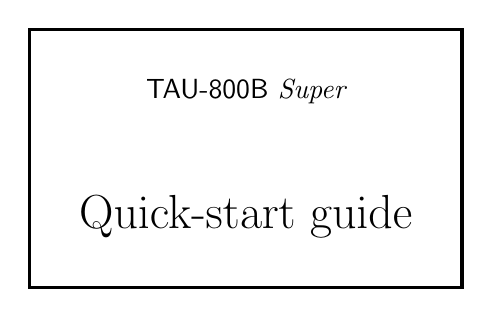
\begin{tikzpicture}
			\node[rectangle,draw,very thick,inner sep=18pt,align=center] {
			{\HUGE \machinename}
			\\[32pt]
			{\LARGE Quick-start guide}
			};
		\end{tikzpicture}

		\vfill

		{\footnotesize \companyname{} \\ \companyname*{}}
	\end{adjustwidth*}
\end{titlingpage}



\thispagestyle{empty}

\begin{footnotesize}
	\noindent
	This is a quick-start guide to your \machinename*{} time-assisted computing machine.
	Please ensure you have thoroughly read and understood the User Manual and the Warranty Disclaimer before attempting to utilize the machine.
	\companyname{} is not responsible for any damages resulting from improper use of the time jump facilities of this machine.
	\vfill
	\warningbox{%
		\textbf{\textsf{Please ensure that the Novikov module has sufficient power
				throughout the operation of the machine. Failure to supply the minimum
				rated power may cause time inconsistency paradoxes.}} \\[2pt]
		In the unlikely case of forced inconsistency contact our hotline \\
		\hfill\textsf{\textbf{1-800-NOTIME}}}
\end{footnotesize}



\clearpage
\renewcommand\cftchapterfont{\ttfamily}
\renewcommand\cftchapterleader{\ttfamily\cftdotfill{.}}  % Bué intuitivo, escuta
\renewcommand\cftchapterpagefont{\ttfamily}
%\show\tableofcontents
\tableofcontents*



\mainmatter
\counterwithout{figure}{chapter}

\section{Introduction}
\vspace*{-20pt}\rule{\textwidth}{0.8pt}

\noindent
Congratulations of becoming the proud owner of a \machinename*{}, the latest technology
in time-based computing. The following document serves as an introduction to the
architecture and operation modes of this time-assisted arithmetic computing unit
as well as to any other extensions offered by \companyname{} compatible with the
\machinename{} that were acquired as part of your commercial agreement.

For more information regarding available computing extension hardware compatible
with your computing unit contact your local \companyname{} sales representative.
Missing documentation of acquired computing extension hardware and advanced time
operation modes of the computing unit can be obtained upon written request with
proof of purchase to \companyname{} Hanshin Main Headquarters.

Please note that this document \underline{does not} preclude the consultation of
the complete reference manual, which should have been provided to you alongside
this document and the computing unit. If the complete reference manual was not provided
to you upon purchase, please contact your local sales representative.

\companyname{} is not liable for damages incurred in the misuse of the equipment
to the extent of but not limited to the operation modes described in this document.

\clearpage
\section{Self-consistent Novikov-Turing Assisted Computing}

The \machinename{} provides new computing advances by exploiting the well-known
Novikov-Turing speedup, schematized in figure \ref{fig:timeline} for convenience.
These modes of operation are seamlessly exposed via the assembly language (see section
\ref{sec:assembly}). Please refer to the complete reference manual for examples
of implementation of some of the known temporal computing speedups.

\begin{figure}[bh]
	\setlength{\fboxsep}{20pt}
	\centerline{%
		\fbox{%
			\includegraphics{assets/timeline.png}%
		}%
	}
	\caption{The Turing-Novikov effect at play in the \protect\machinename{} modes
		of operation. The Novikov stability module (full reference manual, sec. 4,
		fig. 10, schematic 1\,a)), ensures self-consistency in the computing process.}
	\label{fig:timeline}
\end{figure}

The \machinename{} architecture was designed to reproduce as closely as possible
(within technical limits) the theoretical model typically employed for causal-consistency
calculations, so as to facilitate the transposition from theoretical programs with
consistency speedups into operation. In figure \ref{fig:architecture}, a schematic
of a high-level overview of the architecture is presented, where each component
in the schematic broadly encompasses various physical elements of the machine.
For a complete description of these physical elements, please refer to the Service
and Schematics section of the complete reference manual.

\begin{sidewaysfigure}
	\setlength{\fboxsep}{20pt}
	\centerline{%
		\fbox{%
			\includegraphics{assets/architecture.png}%
		}
	}
	\caption{High-level overview of causal-consistent hardware architecture. }
	\label{fig:architecture}
\end{sidewaysfigure}

\clearpage
\section{The Machine Language} \label{sec:assembly}
\vspace*{-20pt}\rule{\textwidth}{0.8pt}

\noindent
The following is a quick-reference guide to \machinename{} assembly language. Please
use ONLY the officially licensed assembler programs by \companyname{}.
\footnote{If you have not been supplied with all 9 (nine) floppy diskettes for installation
	of the assembler, please contact your local sales representative.}

%The CPU word size is 8 bits.

Quick facts:
\begin{itemize}[nosep]
	\item 6-bit word size, 12-bit address space with pageable memory.
	\item 0.66\,MHz clock speed.
	\item Four general purpose word registers.
	\item Six-word stack.
	\item Time jumps of up to 200 clock cycles in any direction.\footnotemark
	\item Memory-mapped IO.
	\item Big endian.
\end{itemize}
%
\footnotetext{
	Note: for jumps of over 80 clock cycles an upgraded SPS-3-6000 power supply
	with at least 6\,kW of peak power output must be provided.
	\textbf{Serious damage may occur if you attempt to use these operations without sufficient power!}
	Please refer to section \ref{sec:power} and the complete reference manual for
	more information.}

\subsection*{CPU registers}

The CPU has a total of 10 (ten) words of register memory.
Of these, 5 (five) words are general-purpose registers
and 5 (five) are special-purpose registers.

The general purpose registers are the following: \ttt{A}, \ttt{BH}, \ttt{BL}, \ttt{CH}, \ttt{CL}.
The latter two pairs of registers can be used to store 2-word values, high word and low word respectively.
These registers are used readable and writable via move and arithmetic-logic instructions.

%Then, the CPU has one flag register \ttt{F}, where each bit has the following meaning (left to right: \ttt{SZ--NC})
%\begin{itemize}
%\item[A]
%\end{itemize}
Then, the CPU has one flag register \ttt{F},
%with the following bits: \verb|N--PZC|, respectively negative, parity, zero, and carry flags. 
%with the following bits: \verb|N---ZC|, respectively negative, zero, and carry flags. 
with the following bits: \verb|NV--ZC|, respectively negative, overflow, zero, and carry flags.
These are set and cleared by arithmetic and logical instructions,
and can be queried by the conditional branch instructions.
The flag register cannot be written to, but it can be read and copied to memory or another register.
\todo{Se calhar é melhor não se copiar e pronto}

The \ttt{X} register is an index register: it can be read and written to like a general purpose register,
%and it can be added as an offset to a location in memory 
and it can be used in the indexed addressing mode to access a location obtained by adding the contents of the register to a base address.

The CPU also has a stack pointer, that points to one-past the top of the stack.
It can be read or written to as a general purpose register, but it is also altered by the \ttt{CAL}, \ttt{RET}, \ttt{PSH}, \ttt{POP} instructions.

Finally, the two-word program counter stores the address of the next instruction, and can be modified by jump, branching and subroutine instructions

12-bit addresses are read and stored as two words in big-endian order: \ttt{\%llhh}.
In order to perform 12-bit arithmetic, you must process the two words manually.\footnotemark

\footnotetext{Advanced mathematical subroutines are available for purchase, please contact your regional sales representative.}

\filbreak % Prefer a break here
\subsection*{Addressing modes}

The following addressing modes are available:

%\begin{itemize}[nosep]
%	\item Register \ttt{\%a}: addresses a named register.
%	\item Immediate \ttt{\#ff}: represents a literal one-word value.
%	\item Immediate \ttt{\#fff}: represents a literal two-word value.
%	\item Absolute \ttt{\%llhh}: the memory address $\ttt{ll}+2^8\ttt{hh}$.
%	\item Indexed \ttt{\%llhh,X}: the memory address $\ttt{ll}+2^8\ttt{hh}+\textrm{contents of \ttt{X}}$.
%	\item Indirect \ttt{(\%llhh)}: the address stored at memory address $\ttt{ll}+2^8\ttt{hh}$.
%	\item Indirect \ttt{(\%b)} \ttt{(\%c)}: the address $\ttt{c}$
%\end{itemize}

% Estas tabelas com linhas em todo o lado são péssimas xD mas faz parte da aesthetic, que achas?
\begin{center}
	\begin{tabular}{|l|l|l|}
		\hline
		\textbf{Mode} & \textbf{Notation}                       & \textbf{Description}                                                    \\ \hline
		Register      & \ttt{\%a}                               & a named register                                                        \\ \hline
		Immediate     & \ttt{\#ff}                              & represents a literal one-word value                                     \\ \hline
		Immediate     & \ttt{\#fff}                             & represents a literal two-word value                                     \\ \hline
		Absolute      & \ttt{\%llhh}                            & the memory address $\ttt{ll}+2^6×\ttt{hh}$                              \\ \hline
		Indexed       & \ttt{\%llhh,X}                          & the memory address $\ttt{ll}+2^6×\ttt{hh}+\textrm{contents of \ttt{X}}$ \\ \hline
		Indirect      & \hspace{-0.2em}\ttt{(\%llhh)}           & the address stored at memory address $\ttt{ll}+2^6×\ttt{hh}$            \\ \hline
		%	Indirect  & \hspace{-0.2em}\ttt{(\%b)}\,\ttt{(\%c)} & the address stored at memory address $\ttt{bh}$ (resp c)\\ \hline
		Indirect      & \hspace{-0.2em}\ttt{(\%r)}\footnotemark & the address stored at memory address $\ttt{rl}+2^6×\ttt{rh}$            \\ \hline
	\end{tabular}
\end{center}

\footnotetext{Where \ttt{r} is \ttt{b} or \ttt{c}.}

\subsection*{List of instructions}

The following is a quick-reference list of instructions.

\newcommand\instruction[2]{%
	\noindent
	\begin{minipage}[t]{0.22\textwidth} \texttt{#1} \end{minipage}
	\hspace{0.03\textwidth}
	\begin{minipage}[t]{0.75\textwidth} #2 \end{minipage}
	%	\medskip
	\vspace*{-0.5\smallskipamount}
}

\noindent
\textit{\small Note: unless otherwise noted, instructions that 「set the \ttt{Z} flag」 set it if the result is zero, and clear it otherwise, instructions that 「set the \ttt{N} flag」 set it to the value of the most significant bit of the result (i.e.\ set if negative, clear otherwise); and instructions that 「set the \ttt{V} flag」  set it to the value of the second most significant bit of the result (i.e.\ set if signed arithmetic overflows, clear otherwise).}.
\subsubsection*{Memory}

\instruction{MOV src dst}{Set word at \texttt{dst} to contents of \texttt{src}. \\ Flags: set \ttt{Z}, \ttt{N}, \ttt{V}.}

\instruction{PSH src}{Push \ttt{src} onto the stack and increment \ttt{sp}.}

\instruction{POP dst}{Pop value on the top of the stack onto \ttt{dst} and decrement \ttt{sp}.}

\subsubsection*{Arithmetic}

\instruction{ADD src dst}{%
	Set word at \texttt{dst} to $\texttt{src}+\texttt{dst}+\ttt{C}$. \\
	Flags: set \ttt{Z}, \ttt{N}, \ttt{V}, set \ttt{C} on overflow.
}

\instruction{SUB src dst}{%
	Set word at \texttt{dst} to $\texttt{src}-\texttt{dst}-\overline{\ttt{C}}$. \\
	Flags: set \ttt{Z}, \ttt{N}, \ttt{V}, set \ttt{C} on underflow.
}

\instruction{MUL src dst}{%
	Set word at \texttt{dst} to $\texttt{src}×\texttt{dst}$, where operands are unsigned values. \\
	Flags: set \ttt{Z}, \ttt{N}, \ttt{V}, set \ttt{C} on overflow.
}

\instruction{MUS src dst}{%
	Set word at \texttt{dst} to $\texttt{src}×\texttt{dst}$, where operands are signed values. \\
	Flags: set \ttt{Z}, \ttt{N}, \ttt{V}, set \ttt{C} on overflow.
}

%\todo{Como fazer handle de divisoes por zero?}
\instruction{DIV src dst}{%
	Set word at \texttt{dst} to $\texttt{src}\div\texttt{dst}$, where operands are unsigned values. \\
	Flags: set \ttt{Z}.
}

\instruction{DIS src dst}{%
	Set word at \texttt{dst} to $\texttt{src}\div\texttt{dst}$, where operands are signed values. \\
	Flags: set \ttt{Z}.
}

\renewcommand\mod%
{\mathrel{\mathrm{mod}}}

\instruction{MOD src dst}{%
	Set word at \texttt{dst} to $\texttt{src}\mod\texttt{dst}$, where operands are unsigned values. \\
	Flags: set \ttt{Z}.
}

\instruction{MOS src dst}{%
	Set word at \texttt{dst} to $\texttt{src}\mod\texttt{dst}$, where operands are signed values.\\
	Flags: set \ttt{Z}.
}


\instruction{AND src dst}{%
	Set word at \ttt{dst} to bitwise-and of \ttt{src} and \ttt{dst}. \\
	Flags: set \ttt{Z}, \ttt{N}, \ttt{V}.
}

\instruction{OR~ src dst}{%
	Set word at \ttt{dst} to bitwise-or of \ttt{src} and \ttt{dst}. \\
	Flags: set \ttt{Z}, \ttt{N}, \ttt{V}.
}

\instruction{XOR src dst}{%
	Set word at \ttt{dst} to bitwise-xor of \ttt{src} and \ttt{dst}. \\
	Flags: set \ttt{Z}, \ttt{N}, \ttt{V}.
}

\instruction{NOT dst}{%
	Set word at \ttt{dst} to bitwise-not of \ttt{dst}. \\
	Flags: set \ttt{Z}, \ttt{N}, \ttt{V}.
}

\instruction{LSL dst}{%
	Shift bits in \ttt{dst} to the left. \\
	Flags: set \ttt{Z}, \ttt{N}, \ttt{V}, set \ttt{C} on overflow.
}

\instruction{LSR dst}{%
	Shift bits in \ttt{dst} to the right. \\
	Flags: set \ttt{Z}, \ttt{N}, \ttt{V}.
}



\subsubsection*{Comparison}

\instruction{CMP src dst}{Flags: set \ttt{C} to $\texttt{src}>\texttt{dst}$, set \ttt{Z} to $\texttt{src}=\texttt{dst}$.}

\instruction{BIT src dst}{Flags: set \ttt{Z} to $\neg(\texttt{src}\land\texttt{dst})$.}
%Set \ttt{N} to msb of $\ttt{src}\land\ttt{dst}$.




\subsubsection*{Jump}

\instruction{JMP addr}{Jump execution to \texttt{addr} (two-word address).}

\subsubsection*{Branching}

\instruction{BCC off}{Branch to $\ttt{pc}+\ttt{off}$ if \ttt{C} clear (signed offset).}

\instruction{BCS off}{Branch to $\ttt{pc}+\ttt{off}$ if \ttt{C} set (signed offset).}

\instruction{BNE off}{Branch to $\ttt{pc}+\ttt{off}$ if \ttt{Z} clear (signed offset).}

\instruction{BEQ off}{Branch to $\ttt{pc}+\ttt{off}$ if \ttt{Z} set (signed offset).}

\instruction{BPL off}{Branch to $\ttt{pc}+\ttt{off}$ if \ttt{N} clear (signed offset).}

\instruction{BMI off}{Branch to $\ttt{pc}+\ttt{off}$ if \ttt{N} set (signed offset).}

\subsubsection*{Control}

\instruction{CLC}{Clear carry flag}

\instruction{SEC}{Set carry flag}

\subsubsection*{Subroutines}

\instruction{CAL dst}{Store current \texttt{pc} in stack, increment \texttt{sp}, and jump to \texttt{dst}.}

\instruction{RET~~~~}{Read \texttt{pc} from stack, decrement \texttt{sp}, and jump.}

\subsubsection*{Miscellaneous}

\instruction{NOP}{No-op.}

\clearpage
\section{Power Consumptions} \label{sec:power}

Fundamental energetic lower bounds are imposed by the Novikov-Carnot-Landauer principle.
Therefore, despite the high efficiency and stability of \companyname{} components,
the \machinename{}'s power consumption is variable with temperature and operation
mode. In figure \ref{fig:power}, we provide for convenience empirical {Power Consumption/Temperature}
curves, obtained in standard conditions. However, \emph{for optimal performance, we recommend
that you characterize your \protect\machinename{} unit, and adjust your power supply to
provide power accordingly}.

\begin{figure}[hbp]
	\centerline{%
		\pdfimageresolution=200
		\includegraphics{assets/power.png}%
	}
	\caption{Experimental power consumptions for varying temperature per operating
		mode of the \protect\machinename{} (Primary Power Supply). Data obtained
		in standard conditions and interpolated to normal distribution.}
	\label{fig:power}
\end{figure}

The Novikov module must be powered separately, typically with a buffer SPS-3-5000
or SPS-3-6000 module between mains and the module. \textbf{To avoid catastrophic
failure, the secondary power supply \emph{must} be able to provide constant minimum
ratings throughout operation}. The SPS-3-* modules provide brown-out detection,
and are therefore highly recommended. The exact required ratings can be found in
the service manual provided separately with the Novikov components. If this manual
was not provided to you, \underline{\textbf{do not}} operate the machine and contact your sales
representative. \emph{Typical} ratings are provided, for convenience, in figure
\ref{fig:novikov-power}.

\begin{sidewaysfigure}[hb]
	\centerline{%
		\pdfimageresolution=200
		\includegraphics{assets/novikov-power.png}%
	}
	\caption{\emph{Typical} power ratings (Secondary Power Supply) for varying temporal
		offsets in the Novikov module. \textbf{These values are for comparison
		\emph{only}}. You \underline{must} characterize and ensure correct
		ratings for your Novikov module. The installation technician should have
		characterized and provided the ratings for your machine in the complete
		reference manual.}
	\label{fig:novikov-power}
\end{sidewaysfigure}

\clearpage
\thispagestyle{empty}
\null\vfill
{\bfseries
\null\hfill\companyname{}\hfill\null

\null\hfill\companyname*{}\hfill\null}
\vfill\null

\centerline{\ttfamily Do not distribute. \copyright*{} 1973}

\end{document}
